\chapter{Dynamic Force Simulation}

In the previous section the calculations at static conditions were described. However, often it is interesting what the maximum forces are during bouncing or jumping. On highlines the forces involved in a leashfall are also very important. As the calculation of dynamic behavior is much more complicated than on static conditions finding analytic expressions is not constructive. Therefore an simulation approach is used.


\section{Basic Idea of the Simulation}
To get the forces on dynamic movements the movement of the slackliner gets separated in very small time steps and for a hole period of bouncing or jumping the current speed and position get calculated for every time step. If the time steps are small enough the acceleration of the slackliner can be assumed to be constant. That leads to the following formulas:

\begin{align}
	v(t) &= at+v_0 \\
	s(t) &= \frac{a}{2}t^2 + v_0 t + s_0
\end{align}

In addition the following relations exists:

\begin{equation}
	F = a\cdot m
\end{equation}

$a$ is the accelaration, $m$ the mass, $v$ the speed and $s$ the path. Then for every time step the following pattern is done:

\begin{enumerate}
	\item Set the sag of the slackline to the current position of  the slackliner
	\item Calculate the force affecting the slackliner $F = m\cdot g - F_{v,slackline}$
	\item Calculate the acceleration of the slackliner $a = F / m$
	\item Calculate change in speed $\Delta v = a\cdot\Delta t$
	\item Calculate change in position $\Delta s = \frac{1}{2}\cdot a\cdot\Delta t^2 + v\cdot\Delta t$
	\item Add those values to the current position and speed
\end{enumerate}

When the sign of the speed changes the slackliner is at the lowest point of the line. At this point the maximum forces on the line and the slackliner appear. Therefore the simulation can be stopped here.

\section{Improved Dynamic Model (not implemented)}

In the section above it is assumed, that the stretch behavior of the line is always the same as in the static case. In reality this is not the case and the line behaves more like a viscoelastic material. Therefore it might lead to better results assuming a model based on viscoelastic behavior for the dynamic simulations.

\begin{figure}[htb] \centering
	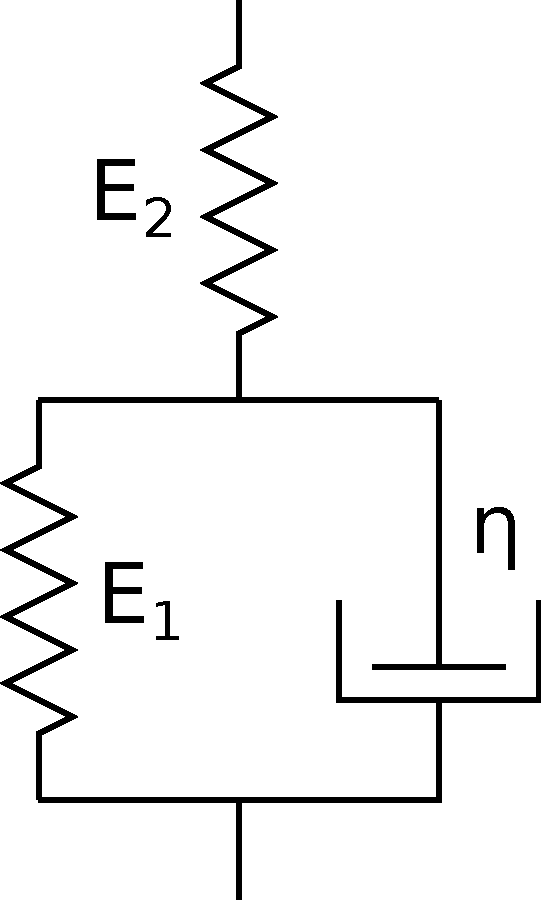
\includegraphics[width=0.4\textwidth]{images/dynamicStandardModel.pdf}
	\caption{Standard linear solid model}
	\label{fig:dynamicStandardModel}
\end{figure}

Figure \ref{fig:dynamicStandardModel} shows the standard linear solid model often used to describe viscoelastic behavior. This leads to the following differential equation:

\begin{equation}
	\sigma + \frac{\eta}{E_1+E_2}\dot\sigma = \frac{E_1E_2}{E_1+E_2}\epsilon + \frac{E_2\eta}{E_1+E_2}\dot\epsilon
	\label{eqn:standardLinearModel}
\end{equation}

$E_1$, $E_2$ are the elastic modulus of the two springs, $\sigma$ is the applied stress, $\epsilon$ is the stretch $\frac{\Delta l}{l}$ and $\eta$ is the dynamic viscosity. 

For the calculation of slacklines I like to use the stretch coefficient $\alpha = \frac{\epsilon}{F}$ instead of the elastic modulus. The relation between those parameters is:

\begin{equation}
	E = \frac{1}{\alpha\cdot A}
\end{equation}

The sum of the stretch coefficients $\alpha_1+\alpha_2$ then is the static stretch coefficient $\alpha$ of the line from the previous chapters. As for slacklines the cross section $A$ is not very important it makes sense to multiply equation \ref{eqn:standardLinearModel} with $A$:

\begin{equation}
F(t) + \frac{\alpha_1\alpha_2}{\alpha}\cdot (\eta A)\cdot\dot F(t) = \frac{\epsilon(t)}{\alpha} + \frac{\alpha_1}{\alpha}\cdot (\eta A)\cdot\dot{\epsilon(t)}
\end{equation}

Rearranging this equation leads to

\begin{equation}
	\dot F(t) = \frac{-\alpha}{\alpha_1\alpha_2\cdot (\eta A)} \cdot F(t) + \frac{\epsilon (t)}{\alpha_1\alpha_2\cdot(\eta A)} + \frac{\dot{\epsilon} (t)}{\alpha_2}
\end{equation}

Now we have a linear inhomogeneous differential equation. Solving this equation for the force $F$ gives:

\begin{equation}
\begin{split}
	F(t) \insertForSmartphone{&}= e^{ \frac{-\alpha t}{\alpha_1\alpha_2\cdot (\eta A)} dt } \cdot \insertForSmartphone{\\ &}\left[ \int_0^t \left( \frac{\epsilon (t')}{\alpha_1\alpha_2\cdot (\eta A)} + \frac{\dot{\epsilon}   (t')}{\alpha_2} \right) \cdot e^{\frac{\alpha t'}{\alpha_1\alpha_2\cdot (\eta A)}} dt' + C \right]
\end{split}
\end{equation}

For the simulation the change of force $\Delta F$ between to time steps $\Delta t$ is of interest. Therefore $\Delta F = F(t+\Delta t) - F(t)$ has to be calculated:

\begin{equation}
\begin{split}
	\Delta F = F(t)\cdot \left( e^{\frac{-\alpha\cdot \Delta t}{\alpha_1\alpha_2\cdot(\eta A)}} - 1 \right) + e^{\frac{-\alpha(t+\Delta t)}{\alpha_1\alpha_2\cdot (\eta A)}} \cdot \insertForSmartphone{\\} \int_t^{t+\Delta t} \left( \frac{\epsilon (t')}{\alpha_1\alpha_2\cdot(\eta A)} + \frac{\dot{ \epsilon} (t')}{\alpha_1} \right) \cdot e^{\frac{\alpha\cdot t'}{\alpha_1\alpha_2\cdot (\eta A)}} dt'
\end{split}
\end{equation}

 If the time steps are small enough a constant stretch $\epsilon(t) = \epsilon = const$ can be assumed for the integration. The derivation of the stretch changes to $\dot{\epsilon}(t) = \frac{\Delta\epsilon}{\Delta t}$. With this simplification the remaining integral can be solved.
The result is:

\begin{equation}
	\Delta F = \left( 1 - e^{\frac{-\alpha\cdot\Delta t}{\alpha_1\alpha_2\cdot (\eta A)}} \right) \cdot \left( \frac{\epsilon}{\alpha} - F(t) + \frac{\alpha_1\cdot (\eta A)}{\alpha} \cdot \frac{\Delta\epsilon}{\Delta t} \right)
	\label{eqn:finalDynamicEquation}
\end{equation}

Equation \ref{eqn:finalDynamicEquation} can now easily be used for the simulation. The calculation of the current forces works with the following procedure.

\begin{enumerate}
	\item Initialize the force with the pretension and the stretch with the force-stretch-diagram
	\item Calculate the new position of the slackliner and sag of the line according to the previous section
	\item Calculate the new stretch and $\Delta\epsilon$ with the geometric properties of the line
	\item Calculate the new force $F(t+\Delta t) = F(t) + \Delta F$ with equation \ref{eqn:finalDynamicEquation}
	\item Repeat steps 2 - 4
\end{enumerate}


To get good simulation results dynamic characterizations of some real lines are necessary. However, as a starting point I could find some dynamic parameters of climbing ropes at the following webpage (unfortunately in german): \url{http://www.sigmadewe.com/fileadmin/user_upload/pdf-Dateien/SEILPHYSIK.pdf}.
For the ropes tested there the ratio $\frac{\alpha_1}{\alpha_2}$ was always about $3$. The viscosity was varying between $\eta A = 4.8 \dots 9\,kN\cdot s$. I can imagine that slacklines might have a lower damping than climbing ropes, but that is only speculation. When I have time I will implement this model and play around with the parameters to see if I can get a good match to existing dynamic force measurements.
